\documentclass[border=10pt]{standalone}
\usepackage{tikz}

\begin{document}
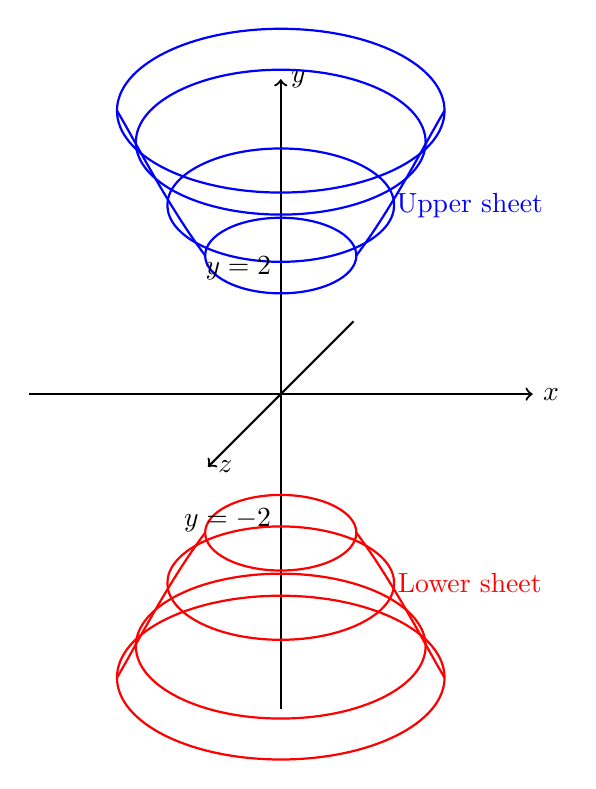
\begin{tikzpicture}[scale=0.8]
% Draw coordinate axes in 3D perspective
\draw[->, thick] (-4,0,0) -- (4,0,0) node[right] {$x$};
\draw[->, thick] (0,-5,0) -- (0,5,0) node[right] {$y$};
\draw[->, thick] (0,0,-3) -- (0,0,3) node[right] {$z$};

% Upper sheet - ellipses at different y levels
\draw[blue, thick] (0,2.2,0) ellipse (1.2 and 0.6);
\draw[blue, thick] (0,3,0) ellipse (1.8 and 0.9);
\draw[blue, thick] (0,4,0) ellipse (2.3 and 1.15);
\draw[blue, thick] (0,4.5,0) ellipse (2.6 and 1.3);

% Lower sheet - ellipses at different y levels
\draw[red, thick] (0,-2.2,0) ellipse (1.2 and 0.6);
\draw[red, thick] (0,-3,0) ellipse (1.8 and 0.9);
\draw[red, thick] (0,-4,0) ellipse (2.3 and 1.15);
\draw[red, thick] (0,-4.5,0) ellipse (2.6 and 1.3);

% Connecting lines to show surface
\draw[blue, thick] (1.2,2.2,0) .. controls (1.8,3,0) and (2.3,4,0) .. (2.6,4.5,0);
\draw[blue, thick] (-1.2,2.2,0) .. controls (-1.8,3,0) and (-2.3,4,0) .. (-2.6,4.5,0);
\draw[red, thick] (1.2,-2.2,0) .. controls (1.8,-3,0) and (2.3,-4,0) .. (2.6,-4.5,0);
\draw[red, thick] (-1.2,-2.2,0) .. controls (-1.8,-3,0) and (-2.3,-4,0) .. (-2.6,-4.5,0);

% Labels
\node[blue] at (3,3,0) {Upper sheet};
\node[red] at (3,-3,0) {Lower sheet};
\node at (0,2,0) [left] {$y=2$};
\node at (0,-2,0) [left] {$y=-2$};

\end{tikzpicture}
\end{document}